\documentclass[18pt]{beamer}
\usepackage[utf8]{inputenc} % for the umlauts

\beamertemplatenavigationsymbolsempty
%% SLIDE FORMAT

% use 'beamerthemekit' for standard 4:3 ratio
% for widescreen slides (16:9), use 'beamerthemekitwide'

\usepackage{templates/beamerthemekit}
% \usepackage{templates/beamerthemekitwide}

\setcounter{tocdepth}{1}

%% TITLE PICTURE

% if a custom picture is to be used on the title page, copy it into the 'logos'
% directory, in the line below, replace 'mypicture' with the 
% filename (without extension) and uncomment the following line
% (picture proportions: 63 : 20 for standard, 169 : 40 for wide
% *.eps format if you use latex+dvips+ps2pdf, 
% *.jpg/*.png/*.pdf if you use pdflatex)

%\titleimage{mypicture}

%% TikZ INTEGRATION

% use these packages for PCM symbols and UML classes
% \usepackage{templates/tikzkit}
% \usepackage{templates/tikzuml}

% the presentation starts here

\usepackage[absolute,overlay]{textpos}
%\usepackage[texcoord,grid,gridunit=mm,gridcolor=red, subgridcolor=green]{eso-pic}
\setbeamercovered{invisible}

\title[SWT1]{Softwaretechnik 1 - 1. Tutorium}
\subtitle{Tutorium 03}
\author{Felix Bachmann}
\date{15.05.2017}

\institute{KIT - Institut für Programmstrukturen und Datenorganisation (IPD)}

% Bibliography

\usepackage[citestyle=authoryear,bibstyle=numeric,hyperref,backend=biber]{biblatex}
\addbibresource{templates/example.bib}
\bibhang1em

\begin{document}

% change the following line to "ngerman" for German style date and logos
\selectlanguage{ngerman}

%title page
\begin{frame}
\titlepage
\end{frame}

%table of contents
\begin{frame}{Themenübersicht}
\tableofcontents
\end{frame}

\section{Organisatorisches}
	\subsection{Keine Lösungen ins Forum!}
	\begin{frame}
		\frametitle{Keine Lösungen ins Forum schreiben!}
		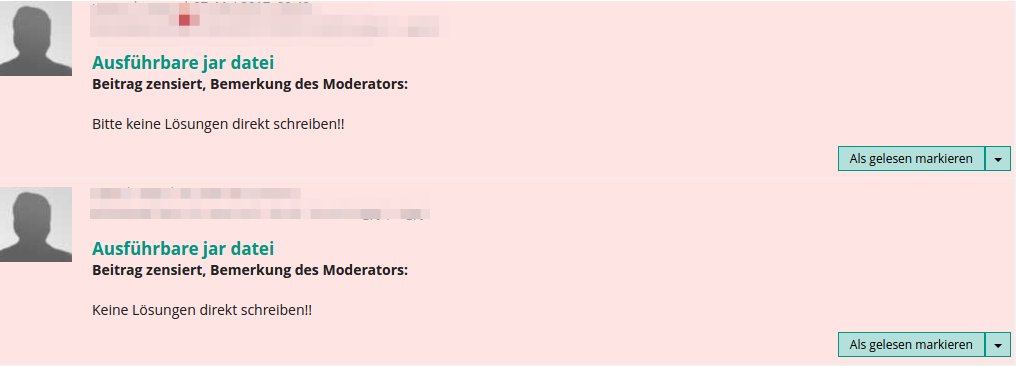
\includegraphics[height=0.85\textheight]{./pics/tut1/censored.png}
	\end{frame}
	
	\subsection{Feedback 1. Übungsblatt}
	\begin{frame}
		\frametitle{1. Übungsblatt Statistik}
		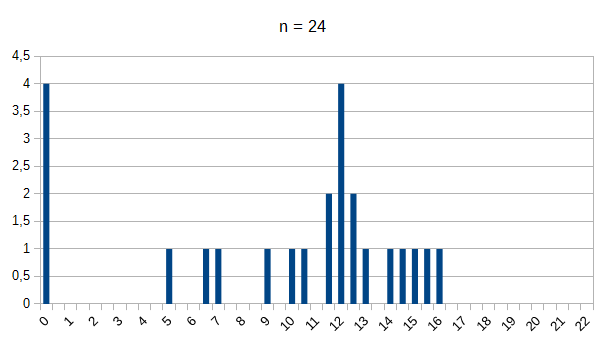
\includegraphics[scale=0.7]{./pics/tut1/statistics_ub1.png}
	\end{frame}
	
	\subsection{1. Übungsblatt - Fehler (Allgemein)}
	\begin{frame}
		\frametitle{Häufige Fehler}
		\begin{block}{Allgemein}
			generell ohne Abzug:
			\begin{itemize}
				\item gleiche Abgabe bei allen Aufgaben
			\end{itemize}
			generell mit Abzug: (bis zu -2P)
			\begin{itemize}
				\item  CheckStyle nicht beachtet
				\item JavaDoc nicht vollständig / nicht aussagekräftig
				\item zu wenige commits / nicht aussagekräftige commit-messages
			\end{itemize}
		\end{block}
	\end{frame}
	
	\subsection{1. Übungsblatt - Fehler (Aufgabe 1)}
	\begin{frame}
		\frametitle{Häufige Fehler}
		\begin{block}{Aufgabe 1 (Altsoftware vorbereiten)}
		\begin{itemize}
			\item *.properties falsch / nicht verschoben (ist Ressource!)
			\item in src.xml wurden *.launch-Dateien nicht hinzugefügt
		\end{itemize}
		\end{block}
	\end{frame}
	
	\subsection{1. Übungsblatt - Fehler (Aufgabe 2)}
	\begin{frame}
		\frametitle{Häufige Fehler}
		\begin{block}{Aufgabe 2 + 3 (Modultests + Testüberdeckung)}
			\begin{itemize}
				\item auch bei Drehung um 0$^{\circ}$  ist Überprüfung des Bildes nötig (Dimensionen + Pixel) \pause
				\item equals() reicht nicht aus, um Gleichheit der Bilder zu prüfen \pause 
				\item new File() erstellt kein File, sondern nur einen "'pointer"' auf einen Pfad (siehe File.createNewFile() oder File.mkdir()) \pause
				\item benutzt relative Pfade (beginnen im jmjrst.main-Ordner) \pause 
				\item Testklasse in gleiches Paket wie zu testenden Klasse \pause 
				\item fügt Abhängigkeiten in die jmjrst.main-pom.xml ein, \textbf{nicht} in die von iMage 
			\end{itemize}
		\end{block}
	\end{frame}

\section{Wasserfallmodell}
	\subsection{Wasserfallmodell, ohne Grafik}
	\begin{frame}
		\frametitle{Wasserfallmodell}
		\begin{itemize}
			\item Was ist das? 
		\end{itemize}
	\end{frame}
	
	\subsection{Wasserfallmodell, mit Grafik}
	\begin{frame}
		\frametitle{Wasserfallmodell}
		dokumentengetriebenes Prozessmodell, das die (möglichen) Phasen der Softwareentwicklung beschreibt
		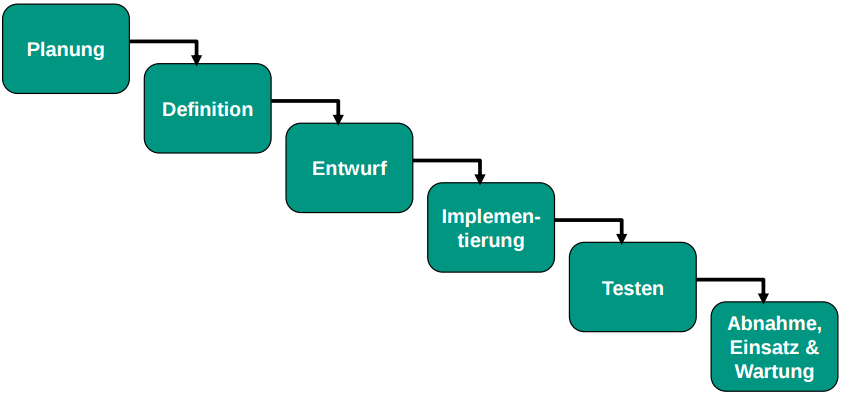
\includegraphics[scale=0.4]{./pics/tut1/waterfall_without-docs.png}
	\end{frame}
	
	\subsection{Wasserfallmodell, mit Grafik und Dokumenten}
	\begin{frame}
		\frametitle{Wasserfallmodell}
		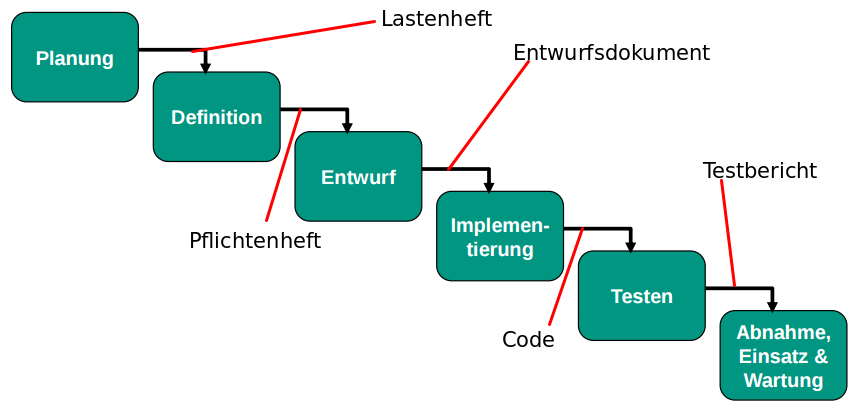
\includegraphics[scale=0.4]{./pics/tut1/waterfall_with-docs.png}
		Dokumente für das 2. ÜB: 
		\begin{itemize}
			\item Lastenheft
			\item Durchführbarkeitsuntersuchung (weiteres Artefakt der Planung)
		\end{itemize}
	\end{frame}

\section{Durchführbarkeitsuntersuchung}
	\subsection{Welche Aspekte?}
	\begin{frame}
		\frametitle{Gliederung}
		\begin{block}{Grundlegende Frage}
			Ist das Projekt in dem jeweiligen Szenario überhaupt durchführbar?
		\end{block}
		\begin{enumerate}
			\item \pause Fachlich \pause 
			\item Alternativen \pause
			\item Personell \pause 
			\item Risiken \pause
			\item Ökonomisch \pause 
			\item Rechtlich 
		\end{enumerate}
		\pause
		\begin{alertblock}{Fürs Übungsblatt}
			Denkt euch was (logisches) aus!
		\end{alertblock}
	\end{frame}

\section{Lastenheft}
	\subsection{Lastenheft - Gliederung}
	\begin{frame}
		\frametitle{Gliederung}
		\begin{block}{Grundlegende Aufgabe}
			Das Lastenheft sammelt die Anforderungen des Auftraggebers an den Auftragnehmer.
		\end{block}
		\begin{enumerate}
			\item \pause Zielbestimmung \pause 
			\item Produkteinsatz \pause
			\item Funktionale Anforderungen \pause 
			\item Produktdaten \pause
			\item Nichtfunktionale Anforderungen \pause 
			\item Systemmodelle
			\begin{itemize}
				\item Szenarien
				\item Anwendungsfälle
			\end{itemize}
			\pause
			\item Glossar 
		\end{enumerate}
	\end{frame}
	
	\subsection{Lastenheft - Unterschiede}
	\begin{frame}
		\frametitle{Begriffsklärung}
		\begin{block}{Zielbestimmung vs. Funktionale Anforderungen}
			\pause
			\begin{itemize}
				\item Zielbestimmung: allgemeine Beschreibung, was das Produkt können soll
				\item Funktionale Anforderungen: konkrete Auflistung von Funktionen
			\end{itemize}
		\end{block}
		\pause
		\begin{block}{Funktionale Anforderungen vs. Nichtfunktionale Anforderungen}
			\pause
			\begin{itemize}
				\item Funktionale Anforderungen: Funktionen des Produkts
				\item Nichtfunktionale Anforderungen: "'Meta"'-Eigenschaften des Produkts
			\end{itemize}
		\end{block}
		\pause
		\begin{block}{Zielbestimmung vs. Produkteinsatz}
			\pause
			\begin{itemize}
				\item Zielbestimmung: allgemeine Beschreibung, was das Produkt können soll
				\item Produkteinsatz: Rahmenbedingungen (Zielgruppe, Anwendungsbereiche)
			\end{itemize}
		\end{block}
	\end{frame}
\section{Pflichtenheft}
%TODO use LaTeX!

%TODO wahr/falsch fragen!

\section{UML-Klassendiagramm}
		
\section{\LaTeX}
		
\section{Tipps}
	\subsection{Tipps}
	\begin{frame}
		\frametitle{Tipps - 2. Übungsblatt}
		\begin{small}
			\begin{exampleblock}{Aufgabe 1}
				%TODO
			\end{exampleblock}
			\pause
			\begin{exampleblock}{Aufgabe 2}
				%TODO
			\end{exampleblock}
			\pause
			\begin{exampleblock}{Aufgabe 3}
				%TODO
			\end{exampleblock}
		\end{small}
	\end{frame}
	
	\subsection{Abgabe}
	\begin{frame}
		\frametitle{Denkt dran!}
		\begin{alertblock}{Abgabe}
			%TODO
		\end{alertblock}
	\end{frame}
		
	\begin{frame}
		\frametitle{Bis dann! (dann=15.05.17)}
		\centering
		%TODO comic \includegraphics[height=0.85\textheight]{}
	\end{frame}

\end{document}
